
\documentclass[a4paper,14pt ]{article} % можно использовать кегель 8-12, 14, 17 и 20 пунктов
\DeclareMathSizes{14}{14}{14}{14}
\usepackage{extsizes}
\usepackage{graphicx}
\graphicspath{{/home/misha/VUZ/TOE/laby/l9}}
\usepackage[russian]{babel} % задаёт русский как основной язык текста
\usepackage[T2A]{fontenc} % задаёт кириллическую кодировку шрифта
\usepackage{cmap} % обеспечивает нормальное копирование и поиск русского текста в pdf 
\usepackage[utf8]{inputenc} % определяет юникодную кодировку самого .tex-файла
\setcounter{secnumdepth}{0}
\usepackage{geometry} % задаёт поля 
\geometry{left=3cm} % левое — 3 см
\geometry{right= 1.5cm} % правое — 1,5 см
\geometry{top=2cm} % верхнее — 2 см
\geometry{bottom=2cm} % нижнее — 2 см
\usepackage{setspace} \onehalfspacing % задаёт «полуторный» межстрочный интервал 
\usepackage{indentfirst} % автоматически добавляет отступ в каждый новый абзац
\usepackage{amsmath,amsfonts,amssymb,amsthm,mathtools,mathtext, physics}
\usepackage{float}
\usepackage{array}
\usepackage{tabularx}
\usepackage{titlesec}
\titleformat{\section}{\centering\normalfont\bfseries}{\thesection}{1em}{}
\titleformat{\subsection}{\centering\normalfont\bfseries}{\thesection}{1em}{}
\titleformat{\subsubsection}{\centering\normalfont\bfseries}{\thesection}{1em}{}
\setlength\parindent{1.25cm}
\begin{document} 
\begin{titlepage}
    \begin{center}
        {\bf  МИНОБРНАУКИ РОССИИ\\
        САНКТ-ПЕТЕРБУРГСКИЙ ГОСУДАРСТВЕННЫЙ\\
        ЭЛЕКТРОТЕХНИЧЕСКИЙ УНИВЕРСТИТЕТ\\
        <<ЛЭТИ>> ИМ. В. И. УЛЬЯНОВА (ЛЕНИНА)\\
    
        }
    \end{center}
    \vfill
        {
        \begin{center}
            \bfseries
            ЛАБОРАТОРНАЯ РАБОТА №3\\
            по дисциплине <<Теоретические основы электротехники>>\\
            Тема: <<ИССЛЕДОВАНИЕ ИНДУКТИВНО СВЯЗАННЫХ ЦЕПЕЙ>>\\
        \end{center}
        }
        \
    \vfill
        {\noindent\parbox{4cm}{Студенты гр. 3114}  \hfill \parbox{3cm}{\rule{3cm}{0.15mm}} \hfill \parbox{4cm}{\raggedleft Злобин М. А.\\ Федулова Л. В. \\ Раузер А. А.}} \\\\
        \parbox{4cm}{Преподаватель} \hfill \parbox{3cm}{\rule{3cm}{0.15mm}} \hfill \parbox{4cm}{\raggedleft Лановенко Е. В.} \\ 
        \center Санкт-Петербург
        
        2025
\end{titlepage}

Цель работы: экспериментальное определение параметров двух индук-
тивно связанных катушек и проверка основных соотношений индуктивно
связанных цепей при различных соединениях катушек.
\section{Определение индуктивностей катушек, взаимной индуктивности
и коэффициента связи}
Расчет параметров катушек осуществляется по формулам 
    \begin{equation}
        \begin{cases}
            x_1 = \omega L_1 = U_1/I_1;
            |x_M| = |\omega M| = U_2/I_1;\\
            x_2 = \omega L_2 = U_2/I_2; |x_M| = U_1/I_2.
        \end{cases}
    \end{equation}
    \indent Первая катушка:\\
    $x_1 = 2/13.3 = 0.151 \, \text{кОм}; $
    $L_1 = x_1/\omega = 0.151/2\pi = 24$ мГн;
    $x_M = 1.45/13.3 = 0.11$ кОм; \\
    $M = 0.11/2\pi = 18$ мГн;\\
    \indent Вторая катушка: \\
    $ x_2 = 2/6.8 = 0.294 \, \text{кОм};$ 
    $L_2 = x_2/\omega = 0.294/2\pi = 47$~мГн \\
    $x_M = 0.72/6.8 = 0.11$ кОм;\\ 
    $M = 0.11/2\pi = 18$ мГн; \\
    \indent Коэффиент связи:\\
    $k = \frac{M}{\sqrt{L_1 L_2}} = 0.11/\sqrt{0.151\cdot 0.294} = 0.52 $;
\section{Исследование последовательного соединения
индуктивно связанных катушек}
    При последвательном соединении $I_1 = I_2$.\\
    \indent Согласное включение:
    $L_{\text{э}} = L_1 + L_2 + 2M = 24 + 47 + 36 = 107 $ мГн.
    \begin{multline}
    \dot{I} = U/Z_{вх} = U/(j\omega(L_1 + L_2 + 2M)) = \\
    = -j\frac{2}{2\pi1000\cdot(L_{\text{э}})} = -j3\, \text{мА}
    \end{multline}
    $\dot{U}_1 = \dot{I}(j\omega L_1 + jM\omega) = 3(0.151+0.11) =0.783$ В.\\
    $\dot{U}_2 =\dot{I}(j\omega L_2 + jM\omega) = 3(0.294 +0.11) = 1.212$ В.\\
    \indent Встречное включение:
    $L_{\text{э}} = L_1 + L_2 - 2M = 24 + 47 - 36 = 37$ мГн. 
    \begin{multline}
    \dot{I} = U/Z_{вх} = U/(j\omega(L_1 + L_2 - 2M)) = \\
    = -j\frac{2}{2\pi1000\cdot(L_{\text{э}})} = -j8.89\, \text{мА}
    \end{multline}
    $\dot{U}_1 = \dot{I}(j\omega L_1 + jM\omega) = 8.89(0.151-0.11) = 0.365$ В.\\
    $\dot{U}_2 =\dot{I}(j\omega L_2 + jM\omega) = 8.89(0.294- 0.11) = 1.636$ В.\\
    \section{Исследование параллельного соединения
индуктивно связанных катушек}
    \indent Согласное включение:\\
    $L_{\text{э}} = \frac{L_1L_2 - M^2}{L_1 + L_2 - 2M} = \frac{0.151 \cdot 0.294 - 0.11^2}{0.151 + 0.294 - 0.22}/2\pi=0.1435/2\pi=23$ мГн;\\
    $\dot{I}_{\text{вх}} = U/j\omega L_{\text{э}} = 1/0.1435 =  -j6.97$ мА; \\
    \indent Встречное включение:\\
    $L_{\text{э}} = \frac{L_1L_2 - M^2}{L_1 + L_2 + 2M} = \frac{0.151 \cdot 0.294 - 0.11^2}{0.151 + 0.294 + 0.22}/2\pi=0.0485/2\pi=7.7$ мГн;\\
    $\dot{I}_{\text{вх}} = U/j\omega L_{\text{э}} = 1/0.0485 =  -j20.61$ мА; \\
\section{Исследование АЧХ функции передачи трансформатора
по напряжению}
    \begin{figure}[H]
        \centering
        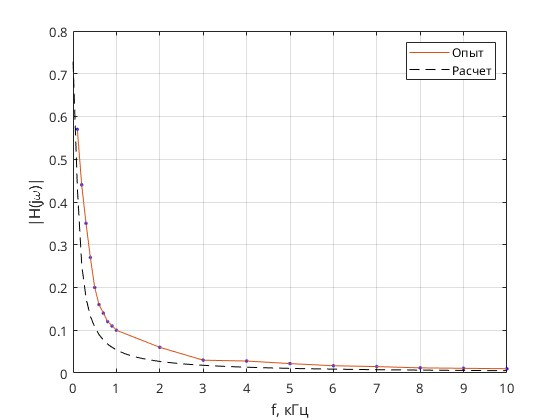
\includegraphics[width=0.75\textwidth]{R_100}
        \caption{АЧХ трансформатора при $R_{\text{н}} = 100$ Ом}
        \label{fig:1}
    \end{figure}

    \begin{figure}[H]
        \centering
        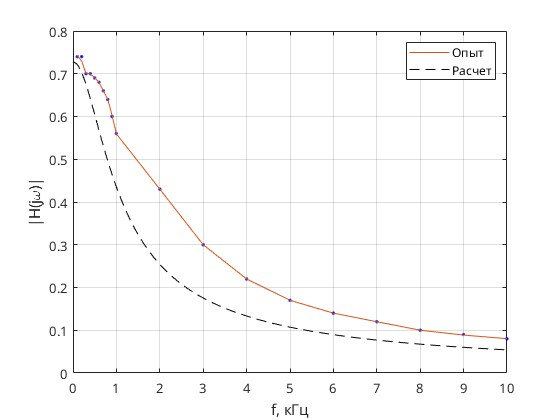
\includegraphics[width=0.75\textwidth]{R_1000}
        \caption{АЧХ трансформатора при $R_{\text{н}} = 1000$ Ом}
        \label{fig:2}
    \end{figure}
    \newpage
    Теоретический расчет АЧХ осуществлялся по формуле
    \begin{equation}
        |H(j\omega)| = \frac{|M|R_{\text{н}}}{\omega \sqrt{{L_1 L_2 - M^2}^2 + (L_1R_{\text{н}}/\omega)^2}}
    \end{equation}
\section{Вопросы}
    \begin{enumerate}
        \item Правильность проведенных экспериментов устанавливается путем сравнения расчетных (теоретических значений) токов и напряжений в катушках,
        со значениями, полученными в ходе эксперимента. Таким образом устанавливается правильность расчета $L_1, L_2, M$.
        \item Чтобы разметить однополярные выводы двух индуктивно связанных катушек, необходимо
        добиться из согласного включения: его характеризует меньший вследствие 
        увеличения эквивалентной индуктивности протекаемый в цепи ток,
        который возможно измерить амперметром. В таком случае катушки соединены разнополярными выводами.
        Соответсвенно, при встречном включении общий ток в цепи будет больше, а катушки будут соединены
        однополярными выводами.
        \item Напряжение на одной из катушек будет отставать от тока при последовательном встречном включении, если коэффициент взаимной индукции \( M \) больше индуктивности этой катушки:

        $ M > L_1 \, \text{(для \( U_1 \))} \, \text{или} \, M > L_2 \, \text{(для \( U_2 \))}. $
        При этом должно выполняться условие физической реализуемости:
        $
        M \leq \sqrt{L_1 L_2}.
        $
        \item При уменьшении частоты индуктивное сопротивление падает, что приводит
        к увеличиению тока и увеличению напряжения на активном сопротивлении обмотки.
        На высоких частотах растет индуктивность рассеяния $L_s$ и сопротивление рассеяния
        $X_s = L_s 2\pi f$, что снижает передачу мощности во вторую обмотку. На нулевой часоте
        АЧХ равно нулю, потому что при постоянном токе отсутствует явление электромагнитной индукции. Трансформатор стремится к идеальному
        в области средних частот (1-2 кГц).
        \item В теоретической формуле отсутствуют активные сопротивления обмоток, которые
        на низких частотах становятся сравнимы с реактивными сопротивлениями. Активные потери при этом 
        становятся велики и значения АЧХ пададают. Также формула предполает постоянность параметров катушек,
        но в реальности они зависят от тока.
    \end{enumerate}
\section{Вывод}
В ходе работы были вычислены параметры катушек $L_1 = 24$ мГн, $L_2 = 47$ мГн и M = 18 мГн.
Были исследованы индуктивно связанные катушки с последовательным и параллельным соединениями, экспериментальные
данные позволили подтвердить правильность расчета параметров катушек, измеренные и расчитанные напряжения (При согласном включении и последовательном соединении:
$U_{1\text{расч}} = 0.78$ В, $U_{1\text{опыт}} = 0.79$ В; $U_{2\text{расч}} = 1.21$ В, $U_{2\text{расч}} = 1.22$ В; при встречном включении:
$U_{1\text{расч}} = 0.36$ B, $U_{1\text{опыт}} = 0.35$ B; $U_{2\text{расч}} = 1.64$ B, $ U_{2\text{опыт}} = 1.62$ В; токи при параллельном соединении и встречном включении:
$I_{1\text{расч}} = 6.97$ A, $U_{1\text{опыт}} = 7.5$ A; при встречном включении: $U_{1\text{опыт}} = 21.2$ мА,
$I_{1\text{расч}} = 20.6$ мА.)
Были измерены и построены АЧХ. Теоретическая кривая АЧХ оказалась ниже опытной из-за 
пренебрежения в теорретической формуле (4) активным сопротивлением обмоток и паразитными емкостями между витками обмотки.
\end{document}